\documentclass[12pt,a4paper]{article}

% (fold)
\usepackage{booktabs,amsmath,multirow} 
\usepackage{mathtools} % needed for next line
\mathtoolsset{showonlyrefs}
\usepackage{fullpage}
 % only shows number of referenced equations
% \newcommand{\dpder}[3][]{\dfrac{\partial^{#1}#2}{\partial #3}} \addtolength{\oddsidemargin}{-.875in} \addtolength{\evensidemargin}{-.875in} \addtolength{\textwidth}{1.75in}
% \addtolength{\topmargin}{-.875in} \addtolength{\textheight}{1.75in}

% need for subequations
\usepackage{graphicx} 

% need for figures
\usepackage{verbatim}

% useful for program l,istings
\usepackage{color} 

% use if color is used in text
\usepackage{subfigure}

% use for side-by-side figures
\usepackage[pdfpagemode={UseOutlines},bookmarks=true,bookmarksopen=true, bookmarksopenlevel=0,bookmarksnumbered=true,hypertexnames=false, colorlinks,linkcolor={blue},citecolor={blue},urlcolor={red}, pdfstartview={FitV},unicode,breaklinks=true]{hyperref} 

% use for hypertext links, including those to external documents and URLs
\newcommand{\ajp}{AJP} 
\newcommand{\ig}{ 
\includegraphics} 
\newcommand{\tu}{\textup} \hypersetup{urlcolor=blue, colorlinks=true} 
\usepackage[square, numbers, comma, sort&compress,super]{natbib}
% Colors hyperlinks in blue - change to black if annoying
% don't need the following. simply use defaults
\setlength{\baselineskip}{16.0pt} 
\usepackage[svgnames]{xcolor}
% 16 pt usual spacing between lines
\begin{comment}
	\pagestyle{empty} 
	
	% use if page numbers not wanted
\end{comment}
\def\Baluminum{0.973} 

\def\Bplastic{0.988} 

\def\chialuminum{9.0} 

\def\chiplastic{31.9} 

\def\dBaluminum{0.0056}

\def\dBplastic{0.046} 

% \def\dRaluminum{3.624} 
{3.163} 
{1.624} 
{3.784} 
{0.515} 
{3.152} 
{3.678} 

% \def\dRplastic{4.356} 
{3.709} 
{3.205} 
{3.011} 
{3.321} 
{1.170} 
{3.407} 

\def\kaluminum{0.442} 

\def\kplastic{0.368} 

\def\dkaluminum{0.002} 

\def\dkplastic{0.002} 

\def\MyWidth{.8\textwidth} % textwidth for multiple graphs
% Specifies the directory where pictures are stored
% above is the preamble (end)

\begin{document} 
%!TEX root = /Users/kevin/SkyDrive/KTH Work/LaTeX Reports/Atomic Nucleus Revised/Atomic Nucleus.tex

%%%%%%%%%%%%%%%%%%%%%%%%%%%%%%%%%%%%%%%%%
% University Assignment Title Page 
% LaTeX Template
% Version 1.0 (27/12/12)
%
% This template has been downloaded from:
% http://www.LaTeXTemplates.com
%
% Original author:
% WikiBooks (http://en.wikibooks.org/wiki/LaTeX/Title_Creation)
%
% License:
% CC BY-NC-SA 3.0 (http://creativecommons.org/licenses/by-nc-sa/3.0/)
% 
% Instructions for using this template:
% This title page is capable of being compiled as is. This is not useful for 
% including it in another document. To do this, you have two options: 
%
% 1) Copy/paste everything between \begin{document} and \end{document} 
% starting at \begin{titlepage} and paste this into another LaTeX file where you 
% want your title page.
% OR
% 2) Remove everything outside the \begin{titlepage} and \end{titlepage} and 
% move this file to the same directory as the LaTeX file you wish to add it to. 
% Then add %!TEX root = /Users/kevin/SkyDrive/KTH Work/LaTeX Reports/Atomic Nucleus Revised/Atomic Nucleus.tex

%%%%%%%%%%%%%%%%%%%%%%%%%%%%%%%%%%%%%%%%%
% University Assignment Title Page 
% LaTeX Template
% Version 1.0 (27/12/12)
%
% This template has been downloaded from:
% http://www.LaTeXTemplates.com
%
% Original author:
% WikiBooks (http://en.wikibooks.org/wiki/LaTeX/Title_Creation)
%
% License:
% CC BY-NC-SA 3.0 (http://creativecommons.org/licenses/by-nc-sa/3.0/)
% 
% Instructions for using this template:
% This title page is capable of being compiled as is. This is not useful for 
% including it in another document. To do this, you have two options: 
%
% 1) Copy/paste everything between \begin{document} and \end{document} 
% starting at \begin{titlepage} and paste this into another LaTeX file where you 
% want your title page.
% OR
% 2) Remove everything outside the \begin{titlepage} and \end{titlepage} and 
% move this file to the same directory as the LaTeX file you wish to add it to. 
% Then add %!TEX root = /Users/kevin/SkyDrive/KTH Work/LaTeX Reports/Atomic Nucleus Revised/Atomic Nucleus.tex

%%%%%%%%%%%%%%%%%%%%%%%%%%%%%%%%%%%%%%%%%
% University Assignment Title Page 
% LaTeX Template
% Version 1.0 (27/12/12)
%
% This template has been downloaded from:
% http://www.LaTeXTemplates.com
%
% Original author:
% WikiBooks (http://en.wikibooks.org/wiki/LaTeX/Title_Creation)
%
% License:
% CC BY-NC-SA 3.0 (http://creativecommons.org/licenses/by-nc-sa/3.0/)
% 
% Instructions for using this template:
% This title page is capable of being compiled as is. This is not useful for 
% including it in another document. To do this, you have two options: 
%
% 1) Copy/paste everything between \begin{document} and \end{document} 
% starting at \begin{titlepage} and paste this into another LaTeX file where you 
% want your title page.
% OR
% 2) Remove everything outside the \begin{titlepage} and \end{titlepage} and 
% move this file to the same directory as the LaTeX file you wish to add it to. 
% Then add \input{./title_page_1.tex} to your LaTeX file where you want your
% title page.
%
%%%%%%%%%%%%%%%%%%%%%%%%%%%%%%%%%%%%%%%%%

%----------------------------------------------------------------------------------------
%	PACKAGES AND OTHER DOCUMENT CONFIGURATIONS
%----------------------------------------------------------------------------------------


\begin{titlepage}

\newcommand{\HRule}{\rule{\linewidth}{0.5mm}} % Defines a new command for the horizontal lines, change thickness here

\center % Center everything on the page
 
%----------------------------------------------------------------------------------------
%	HEADING SECTIONS
%----------------------------------------------------------------------------------------
\textcolor{Navy}{
\textsc{\LARGE KTH Royal Institute of Technology}}\\[1.5cm] % Name of your university/college

\textsc{\Large Modern Physics Lab Report}\\[0.5cm] % Major heading such as course name
% \textsc{\large Minor Heading}\\[0.5cm] % Minor heading such as course title

%----------------------------------------------------------------------------------------
%	TITLE SECTION
%----------------------------------------------------------------------------------------

\HRule \\[0.4cm]
{ \huge \bfseries Atomic Nucleus}\\[0.4cm] % Title of your document
\HRule \\[1.5cm]
 
%----------------------------------------------------------------------------------------
%	AUTHOR SECTION
%----------------------------------------------------------------------------------------

\begin{minipage}{0.4\textwidth}
\begin{flushleft} \large
\emph{Authors:}\\
Kevin \textsc{Mead}~~~871020-3277\\% Your name 
Zhenping \textsc{Lin}~~921106-T065 % Your name
\end{flushleft}
\end{minipage}
~
\begin{minipage}{0.4\textwidth}
\begin{flushright} \large
\emph{Lab Instructors:} \\
Victor \textsc{Mikhalev} \\ % Lab Instructor's Name
Edvin \textsc{Sidebo}
\end{flushright}
\end{minipage}\\[4cm]

% If you don't want a supervisor, uncomment the two lines below and remove the section above
%\Large \emph{Author:}\\
%John \textsc{Smith}\\[3cm] % Your name

%----------------------------------------------------------------------------------------
%	DATE SECTION
%----------------------------------------------------------------------------------------

{\large \today}\\[3cm] % Date, change the \today to a set date if you want to be precise

%----------------------------------------------------------------------------------------
%	LOGO SECTION
%----------------------------------------------------------------------------------------

%\includegraphics{Logo}\\[1cm] % Include a department/university logo - this will require the graphicx package
 
%----------------------------------------------------------------------------------------

\vfill % Fill the rest of the page with whitespace

\end{titlepage} to your LaTeX file where you want your
% title page.
%
%%%%%%%%%%%%%%%%%%%%%%%%%%%%%%%%%%%%%%%%%

%----------------------------------------------------------------------------------------
%	PACKAGES AND OTHER DOCUMENT CONFIGURATIONS
%----------------------------------------------------------------------------------------


\begin{titlepage}

\newcommand{\HRule}{\rule{\linewidth}{0.5mm}} % Defines a new command for the horizontal lines, change thickness here

\center % Center everything on the page
 
%----------------------------------------------------------------------------------------
%	HEADING SECTIONS
%----------------------------------------------------------------------------------------
\textcolor{Navy}{
\textsc{\LARGE KTH Royal Institute of Technology}}\\[1.5cm] % Name of your university/college

\textsc{\Large Modern Physics Lab Report}\\[0.5cm] % Major heading such as course name
% \textsc{\large Minor Heading}\\[0.5cm] % Minor heading such as course title

%----------------------------------------------------------------------------------------
%	TITLE SECTION
%----------------------------------------------------------------------------------------

\HRule \\[0.4cm]
{ \huge \bfseries Atomic Nucleus}\\[0.4cm] % Title of your document
\HRule \\[1.5cm]
 
%----------------------------------------------------------------------------------------
%	AUTHOR SECTION
%----------------------------------------------------------------------------------------

\begin{minipage}{0.4\textwidth}
\begin{flushleft} \large
\emph{Authors:}\\
Kevin \textsc{Mead}~~~871020-3277\\% Your name 
Zhenping \textsc{Lin}~~921106-T065 % Your name
\end{flushleft}
\end{minipage}
~
\begin{minipage}{0.4\textwidth}
\begin{flushright} \large
\emph{Lab Instructors:} \\
Victor \textsc{Mikhalev} \\ % Lab Instructor's Name
Edvin \textsc{Sidebo}
\end{flushright}
\end{minipage}\\[4cm]

% If you don't want a supervisor, uncomment the two lines below and remove the section above
%\Large \emph{Author:}\\
%John \textsc{Smith}\\[3cm] % Your name

%----------------------------------------------------------------------------------------
%	DATE SECTION
%----------------------------------------------------------------------------------------

{\large \today}\\[3cm] % Date, change the \today to a set date if you want to be precise

%----------------------------------------------------------------------------------------
%	LOGO SECTION
%----------------------------------------------------------------------------------------

%\includegraphics{Logo}\\[1cm] % Include a department/university logo - this will require the graphicx package
 
%----------------------------------------------------------------------------------------

\vfill % Fill the rest of the page with whitespace

\end{titlepage} to your LaTeX file where you want your
% title page.
%
%%%%%%%%%%%%%%%%%%%%%%%%%%%%%%%%%%%%%%%%%

%----------------------------------------------------------------------------------------
%	PACKAGES AND OTHER DOCUMENT CONFIGURATIONS
%----------------------------------------------------------------------------------------


\begin{titlepage}

\newcommand{\HRule}{\rule{\linewidth}{0.5mm}} % Defines a new command for the horizontal lines, change thickness here

\center % Center everything on the page
 
%----------------------------------------------------------------------------------------
%	HEADING SECTIONS
%----------------------------------------------------------------------------------------
\textcolor{Navy}{
\textsc{\LARGE KTH Royal Institute of Technology}}\\[1.5cm] % Name of your university/college

\textsc{\Large Modern Physics Lab Report}\\[0.5cm] % Major heading such as course name
% \textsc{\large Minor Heading}\\[0.5cm] % Minor heading such as course title

%----------------------------------------------------------------------------------------
%	TITLE SECTION
%----------------------------------------------------------------------------------------

\HRule \\[0.4cm]
{ \huge \bfseries Atomic Nucleus}\\[0.4cm] % Title of your document
\HRule \\[1.5cm]
 
%----------------------------------------------------------------------------------------
%	AUTHOR SECTION
%----------------------------------------------------------------------------------------

\begin{minipage}{0.4\textwidth}
\begin{flushleft} \large
\emph{Authors:}\\
Kevin \textsc{Mead}~~~871020-3277\\% Your name 
Zhenping \textsc{Lin}~~921106-T065 % Your name
\end{flushleft}
\end{minipage}
~
\begin{minipage}{0.4\textwidth}
\begin{flushright} \large
\emph{Lab Instructors:} \\
Victor \textsc{Mikhalev} \\ % Lab Instructor's Name
Edvin \textsc{Sidebo}
\end{flushright}
\end{minipage}\\[4cm]

% If you don't want a supervisor, uncomment the two lines below and remove the section above
%\Large \emph{Author:}\\
%John \textsc{Smith}\\[3cm] % Your name

%----------------------------------------------------------------------------------------
%	DATE SECTION
%----------------------------------------------------------------------------------------

{\large \today}\\[3cm] % Date, change the \today to a set date if you want to be precise

%----------------------------------------------------------------------------------------
%	LOGO SECTION
%----------------------------------------------------------------------------------------

%\includegraphics{Logo}\\[1cm] % Include a department/university logo - this will require the graphicx package
 
%----------------------------------------------------------------------------------------

\vfill % Fill the rest of the page with whitespace

\end{titlepage}
%\affiliation{KTH Royal Institute of Technology, Electrotechnical Modelling} \email{kmead@kth.se
\newpage
\tableofcontents
\newpage
% \doublespacing
%!TEX root = /Users/kevin/SkyDrive/KTH Work/LaTeX Reports/Atomic Nucleus Revised/Atomic Nucleus.tex

\section{Introduction} % (fold)
\label{sec:introduction}
In this lab, we studied the radioactive materials Cesium-137 and Strontium-90.  Like all radioactive materials, they have unstable nuclei and decay over time through different particle emissions.  There are three main decay processes: alpha, beta, and gamma.  This lab focuses on beta decay and evaluates the ability of these particles to penetrate through both aluminium and plastic.

% section introduction (end)

\section{Theory} 

% (fold)
\label{sec:theory} In both of these radioactive isotopes, beta and gamma decay are present. The beta decay in Cesium and Strontium are both $\beta^-$ decay, as opposed to $\beta^+$, and is given by 

\begin{equation}
	^{A}_{Z}P \to _{Z-1}^{~~~A}D + \beta^- + \bar{\nu}_e \nonumber 
\end{equation}%(beta decay equation)

where $P$ and $D$ represent the parent and daughter atoms and $ \bar{\nu}_e$ is an anti-neutrino. The anti-neutrino is important because it shares the total energy with the beta particle. This leads to a continuous distribution of energies instead of discrete values, see Figure~\ref{fig:Figures_betabi210}.

\begin{figure}
	[bp] \centering 
	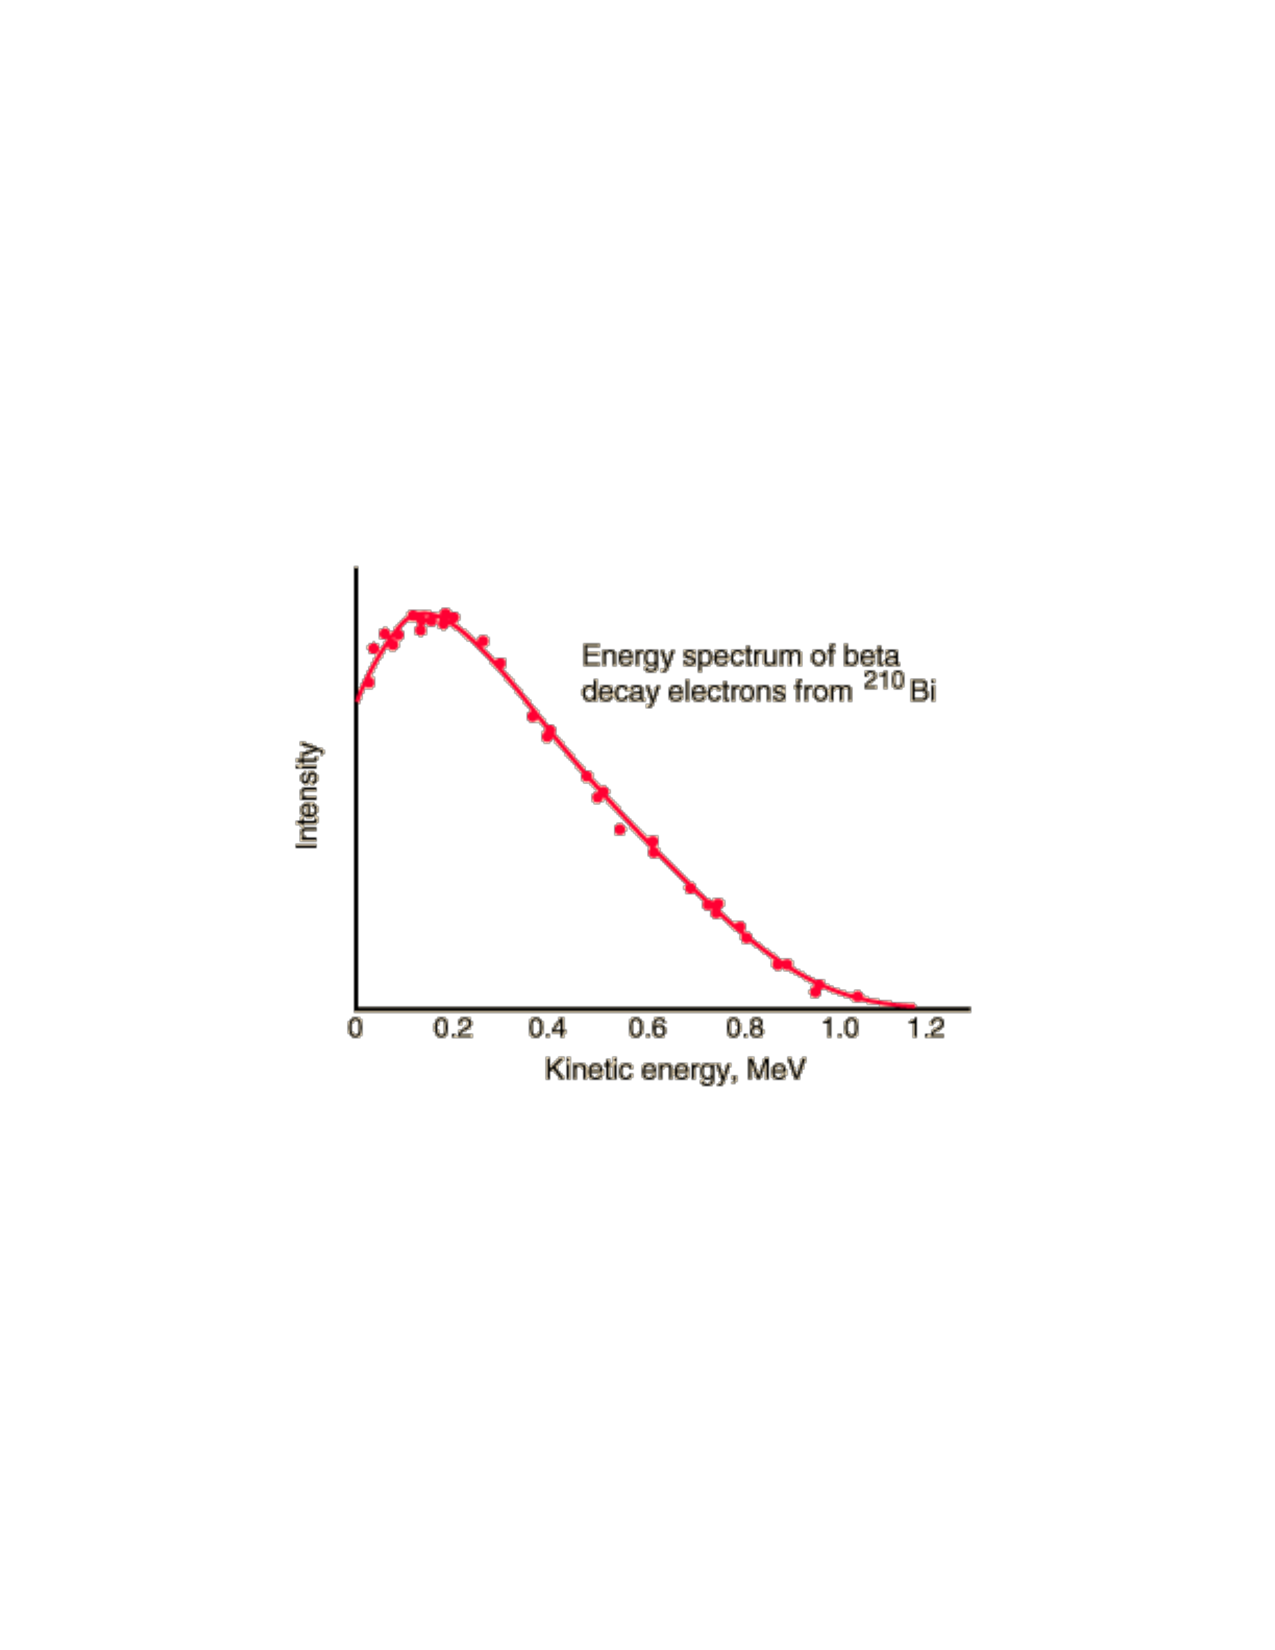
\includegraphics[width=.5
	\textwidth]{./Figures/betabi210.pdf} \caption{General beta decay energy distribution\cite{Neary28031940}} \label{fig:Figures_betabi210} 
\end{figure}%(General Beta Energy Distribution)

Figure~\ref{fig:Figures_137CsDecayScheme} shows the beta decay of cesium with probabilities of each process.
\begin{figure}
	[tbp] \centering 
	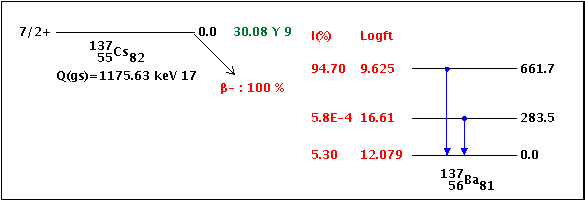
\includegraphics[width=.9
	\textwidth]{./Figures/137CsDecayScheme.png} \caption{Decay Scheme of $^{137}\textrm{Cs}$.\cite{nndc}} \label{fig:Figures_137CsDecayScheme} 
\end{figure}%(fig:Figures_137CsDecayScheme)
Each of these energies must be seen as the maximum energy a beta particle can have because it shares the total energy with an anti-neutrino. From these energies and associated probabilities, we can expect an energy distribution containing one gaussian distribution and two beta distributions with different maximum energy values. Internal conversion occurs $10\%$ of the time at an excited state of Barium, $E=661.7~$keV in Figure~\ref{fig:Figures_137CsDecayScheme}. The other $90\%$ of the time, gamma rays will be emitted. Internal conversion means that an orbiting electron receives the excess energy from a transition between states in the same nucleus $E=661.7~\text{keV}-E_b$, where $E_b=37.441~\text{keV}$ is the binding energy of the electron. It is emitted with an exact amount of energy every time, $E=624.3~\text{keV}$.  However, the collected data will be a normally distributed because of the errors in the measurement equipment and the different path lengths for each electron due to scattering.  

In Figures~\ref{fig:Figures_137CsDecayScheme}, \ref{fig:Figures_90SrDecay}, and \ref{fig:Figures_90YDecay}, I(\%) is the radiation intensity and indicates the probability of occurence.  Logft is given by, $\log(f(Z,E_0)t_{1/2})$, where $f(Z,E_0)$ is the fermi integral, $E_0$ is the end point energy, and $t_{1/2}$ is the half-life.  This value classifies $\beta$ transitions and depends on the probability of decay, half-life, and energy.\cite{nndc} 

A similar beta decay process occurs for Strontium, except it decays through two elements before becoming stable. Both of these decay processes emit beta particles, but does not have internal conversion. First, Strontium decays to Yttrium, $^{90}\text{Y}$, another radioactive isotope (see Figure~\ref{fig:Figures_90SrDecay}). Yttrium then decays to a stable isotope of Zirconium, $^{90}\text{Zr}$ (see Figure~\ref{fig:Figures_90YDecay}).

\begin{figure}
	[tbp] \centering 
	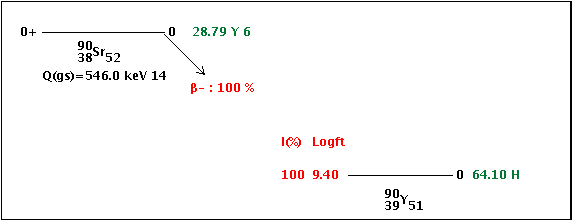
\includegraphics[width=.9
	\textwidth]{Figures/90SrDecay.png} \caption{Decay Scheme of Strontium} \label{fig:Figures_90SrDecay} 
\end{figure}%(fig:Figures_90SrDecay)
\begin{figure}
	[tbp] \centering 
	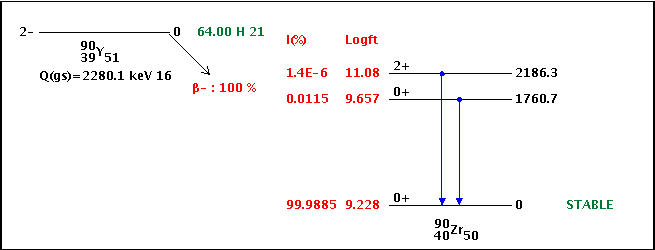
\includegraphics[width=.9
	\textwidth]{Figures/90YDecay.png} \caption{Decay Scheme of Yttrium.  Two of the three decay processes shown have extremely low probabilities ($\ll 1\%$) and therefore, the only process considered has an energy, $\text{E}=2280.1~\text{keV}$.} \label{fig:Figures_90YDecay} 
\end{figure}%(fig:Figures_90YDecay)

% Repeat for decay processes of Strontium except it has two decay processes that occur. Cesium produces a discrete energy value at \textbf{value} This property of Cesium is used in the experimental setup for calibration. 

From this energy distribution, we can determine the beta particles ability to penetrate materials and in this experiment we will use aluminium and plastic. We adjust the thickness of the material and the material to determine a thickness needed to stop beta particles of a certain energy. Every time we add thickness to the materials, we expect the energy distributions to shift towards lower energies.  We expect a shift towards lower energies because they will lose energy due to elastic collisions and rarely will they reflect $180^\circ$.  On the other hand, photons will either become absorbed, reflected, or transmitted.  The energy wouldn't shift towards lower energies, but the number of counts collected would decrease with more sheets.
% In this experiment, we will also make the assumption that the electrons take a direct path from the radioactive material to the detector. 


% section theory (end)
%!TEX root = /Users/kevin/SkyDrive/KTH Work/LaTeX Reports/Atomic Nucleus Revised/Atomic Nucleus.tex
\section{Experimental Setup} 

% (fold)
\label{sec:experimental_setup} The two main decay processes in this experiment are gamma and beta. Since we would only like to study beta decay, we have to eliminate the detection of gamma particles. Gamma particles penetrate materials much further than beta particles. By choosing the scintillator in configuration 2, we have a smaller distance over which to absorb and detect radiation. Therefore, this scintillator will detect the beta particles and allow the majority of gamma particles to pass through undetected. It takes more material to stop gamma particles than electrons because gamma particles have a lower probability to interact with materials.  This allows them to travel large distances without any interactions(or loss in energy).

To calibrate the scintillator, we used the discrete energy value given from Cesium's internal conversion, $E=624.3~\text{eV}$. Table~\ref{tab:calibrationNumbers} shows the values we used to calibrate our system from channel numbers to energy values.  The naive assumption was made that the zero channel corresponds to zero energy because we did not have any other known values like the discrete energy given from $^{137}\text{Cs}$. This possible source of error is addressed in Section~\ref{sec:discussion_conclusion}, Discussion/Conclusion.
\begin{table}
	[tbp] 
	\begin{center}
		\begin{tabular}
{ll} \toprule Channel Number & Corresponding Energy\\
                \midrule $0$ &        $0~\text{eV}$\\
                      $1838$ &    $624.3~\text{keV}$\\
\bottomrule 
		\end{tabular}
	\end{center}
	\caption{The values we used to calibrate our system in order to relate channel numbers to energy values.} \label{tab:calibrationNumbers} 
\end{table}%(tab:calibrationNumbers)


% section experimental_setup (end)

\section{Experimental Method} % (fold)
\label{sec:experimental_method}

The description below describes our procedure after calibration of the equipment ($n$ goes from $ 0 \to 6$ for aluminum and $0 \to 5 \text{~and~} 7$, for plastic). For plastic, $n=6$ was skipped only because time was limited.   
% In hindsight, we should have followed some criteria to determine whether or not a peak is distinguishable, instead of ``eyeballing'' it.  
\begin{enumerate}
	\item Place $n$ sheets of absorbing material (aluminum or plastic) between $^{137}\text{Cs}$ and the detector.
	\item Run PC program Multi Channel Analyser Tukan to collect a set number of counts for each measurement. The measurement with aluminum did not use this criteria, only plastic.
	\item Estimate peak center and error by taking the average of the left and right peak estimations.
	\item Obtain list of energies and thicknesses of absorbing material.
	\item Estimate the thickness needed to stop beta particles ($E\approx0$) using a linear approximation.
	\item Estimate and plot $R(E)=\text{k}E^{\text{B}}$, where k and B are constants and $R(E)$ is the length of material needed to stop an electron of energy $E$.
    Estimation of the stopping distance is done by assuming a linear relationship between number of sheets and electron energy.  As more sheets are added, the energies of the collected electrons become smaller and less frequent as they are being scattered from collisions with the absorbing material.
	\item Compare results with similar experiments.\cite{RevModPhys.24.28,nistData}
\end{enumerate}%(Steps for experiment)

% section experimental_method (end)


\section{Results} % (fold)
\label{sec:results}
The peaks of each measurement was recorded in Table~\ref{tab:dataCollected} and Figure~\ref{fig:Figures_aluminumShiftsPlot} and \ref{fig:Figures_plasticShiftsPlot} show the energy distributions from both absorbers while collecting data from $^{137}\text{Cs}$.
\begin{figure}[tbp]
	\centering
		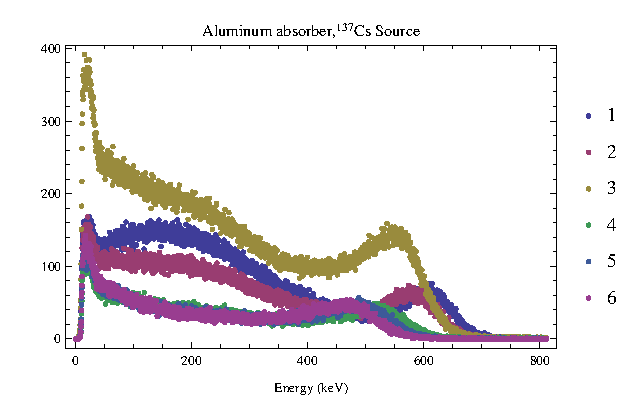
\includegraphics[width=\MyWidth]{Figures/aluminumShiftsPlot.eps}
	\caption{The peaks also shift towards lower energies for aluminum. In order to normalize their intensities, the data for sheets 4,5, and 6 have a constraint on the maximum number of counts collected.  The numbers 1-6 in the plot above and 1-5,7 in Figure~\ref{fig:Figures_plasticShiftsPlot} represent the number of sheets between the radioactive isotope and the scintillator.}
	\label{fig:Figures_aluminumShiftsPlot}
\end{figure}%(fig:Figures_aluminumShiftsPlot)
\begin{figure}[tbp]
	\centering
		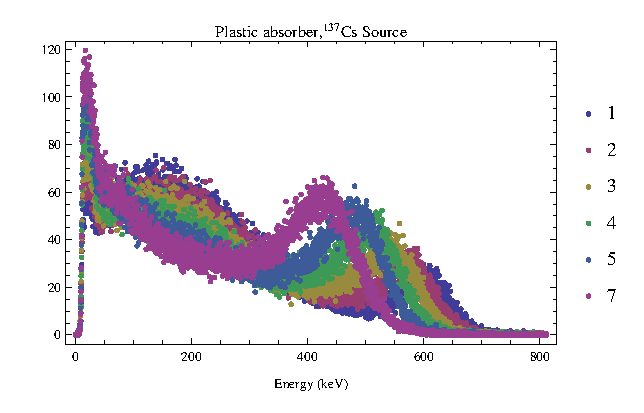
\includegraphics[width=\MyWidth]{Figures/plasticShiftsPlot.eps}
	\caption{The peak of $^{137}\text{Cs}$ shifts towards lower energies as more absorbers are added.  The system was programmed to run until a set number of counts were collected.  The sum of three spectrums shown above contain: the beta spectrum of max energy $1175.63~\text{keV}$ (5\%), the beta spectrum of max energy $513.93~\text{keV}$ (95\%), and the gaussian distribution with a center at $624.3~\text{keV}$ (10\%).}
	\label{fig:Figures_plasticShiftsPlot}
\end{figure}%(fig:Figures_plasticShiftsPlot)
\begin{table}
	[tbp] 
	\begin{center}
		\begin{tabular}{lrrrr}
\toprule
 	 &  		\multicolumn{2}{c}{Aluminum} 			 & 			\multicolumn{2}{c}{Plastic} 				\\
\cmidrule(r){2-3}
\cmidrule(r){4-5}
n    & ($\text{peak}\pm\sigma$)~[keV] 	& Thickness (cm) & ($\text{peak}\pm\sigma$)~[keV] 	& Thickness (cm) 	\\
\midrule
0    & $624.259\pm3$					&	0	         &	$624.259\pm3$					&	0   			\\
1    & $601\pm4$						&	0.0054		 &	$591.5\pm6.5$					&	0.01			\\
2    & $577.5\pm1.5$					&	0.0108		 &	$567.5\pm5.5$					&	0.02			\\
3    & $550.5\pm7.5$					&	0.0162		 &	$537.5\pm6.5$					&	0.03			\\
4    & $505.5\pm1.5$					&	0.0216		 &	$501\pm9$						&	0.04			\\
5    & $470.5\pm8.5$					&	0.027	     &	$470.5\pm4.5$					&	0.05			\\
6    & $450.5\pm10.5$					&	0.0324		 &	\textit{N/A}					&	\textit{N/A}	\\
7    & 	\textit{N/A}	    			&	\textit{N/A} &	$413\pm13$						&	0.07  			\\
\bottomrule
		\end{tabular}
	\end{center}
	\caption{Data collected shows our estimated peaks with standard deviations from taking the average of two possible peaks, one low energy and one high energy.} \label{tab:dataCollected}
\end{table}%(tab:dataCollected)
The electron range, $R(E)$, is interpolated using a linear fit of thickness as a function of energy with the weights $1/\sigma^2$ from Table~\ref{tab:dataCollected}. We fit the function to the equation $R(E)=kE^B$, using a least squares fit.  We used a change of variables to transform our equation into a linear problem,
\begin{align}
	\begin{matrix}
		y = m x + c 	 						\\
		\ln(R(E)) = y 	& 	\mathrm{d}y = \mathrm{d}R/R				\\
		\ln(E) = x 		& 	\mathrm{d}x = \mathrm{d}E/E				\\
		\ln(k) = c 		& 	\mathrm{d}c = \mathrm{d}k/k				\\
		B = m 			& 	\mathrm{d}m = \mathrm{d}B				\\
	\end{matrix}
	\label{eq:transformationEquations}
\end{align}


 Our chi-squared value for aluminum and plastic are $\chialuminum$ and $\chiplastic$, where $\text{N}-2 =5$.  For a good fit, we want $\chi^2\approx \text{N}-2$.  If $\chi^2 \gg \text{N}-2$, it suggests that we are either using the wrong function or our error bars are too small.  If $\chi^2 \ll \text{N}-2$, it suggests that the data fits so well that maybe our error bars are too large.\cite{garcia2000numerical}  We believe the function fit to our data sufficiently describes the range in this domain, but not outside of it.  
 The values for $k$ and $B$ of aluminium are obtained are: $k = \kaluminum \pm \dkaluminum$ and $B = \Baluminum \pm \dBaluminum$. The values for $k$ and $B$ of plastic are: $k = \kplastic \pm \dkplastic$ and $B = \Bplastic \pm \dBplastic$.  These error bars for aluminum are significantly too small, while the error bars for plastic are too large.  Figure~\ref{fig:Figures_linearAluminumGraph} and Figure~\ref{fig:Figures_linearPlasticGraph} give us a better view of the error bars because they plot $\ln(R(E)) vs \ln(E)$, with transformations given in Equation~\eqref{eq:transformationEquations} .

 $R(E)$ has units of g/cm$^2$, making the values independent of the absorbing material. Figure~\ref{fig:Figures_alum_plas_NIST_plot} shows our results compared to two other credible sources\cite{RevModPhys.24.28,nistData}, each with uncertainties around 5\%.  

\begin{comment}
	\begin{figure}[tbp]
		\centering
			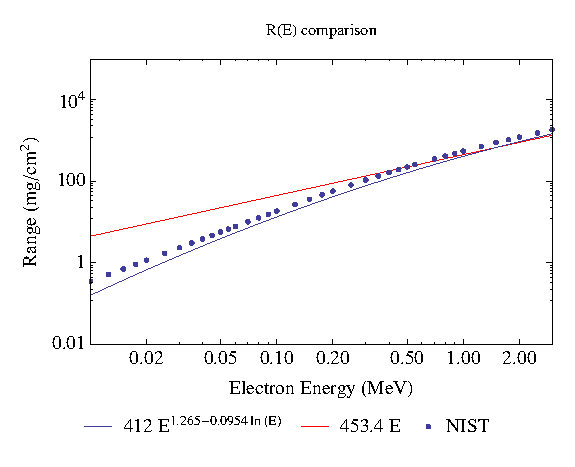
\includegraphics[width=\MyWidth]{Figures/R_E_Comparison.eps}
		\caption{The data we collected agrees with those collected from different sources at higher energies and gets less accurate at lower energies.}
		\label{fig:Figures_R_E_Comparison}
	\end{figure}%fig:Figures_R_E_Comparison
\end{comment}

\begin{figure}[htbp]
  \centering 
  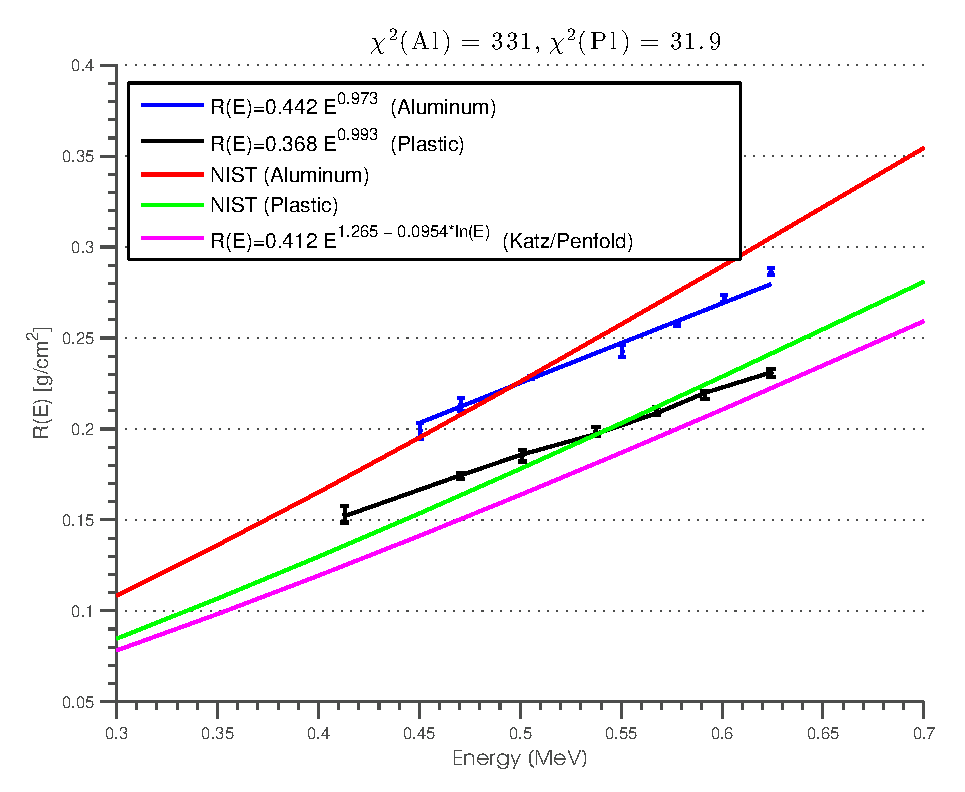
\includegraphics[width=\MyWidth]{Figures/alum_plas_NIST_plot.eps}
  \caption{Comparison of data from aluminum and plastic with accepted values.}
  \label{fig:Figures_alum_plas_NIST_plot}
\end{figure}%(fig:Figures_alum_plas_NIST_plot)

\begin{figure}[htbp]
  \centering
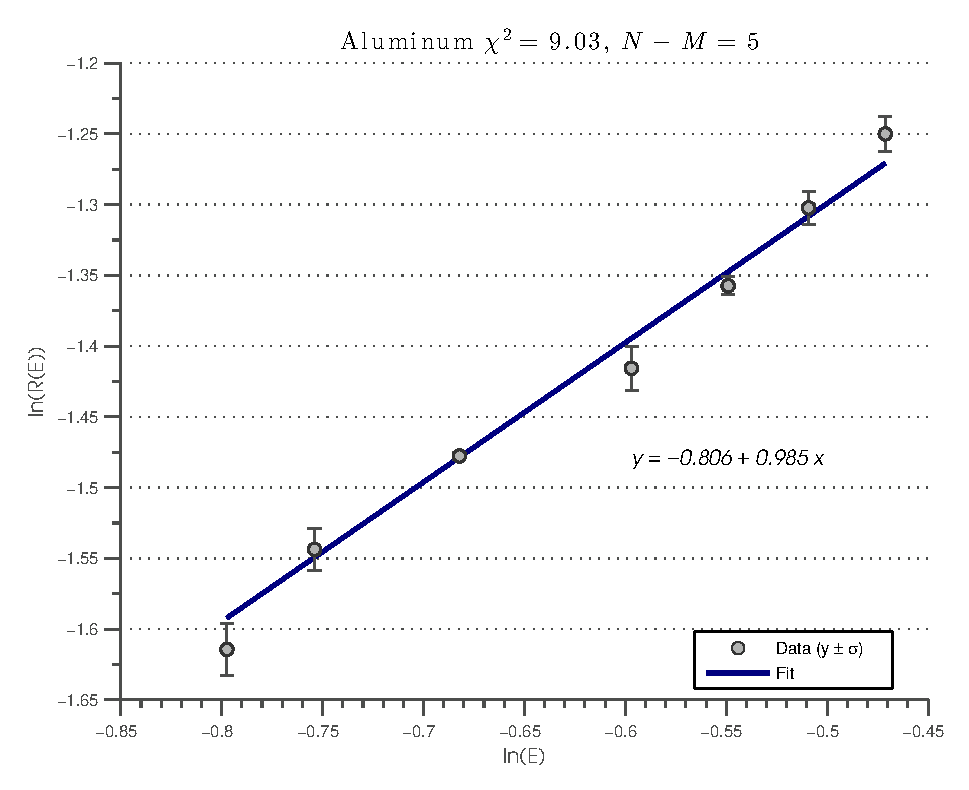
\includegraphics[width=\MyWidth]{Figures/linearAluminumGraph.eps}
  \caption{Graph of aluminum data. $\ln(R(E))$ vs $\ln(E)$}
  \label{fig:Figures_linearAluminumGraph}
\end{figure}%(fig:Figures_linearAluminumGraph)

\begin{figure}[htbp]
  \centering
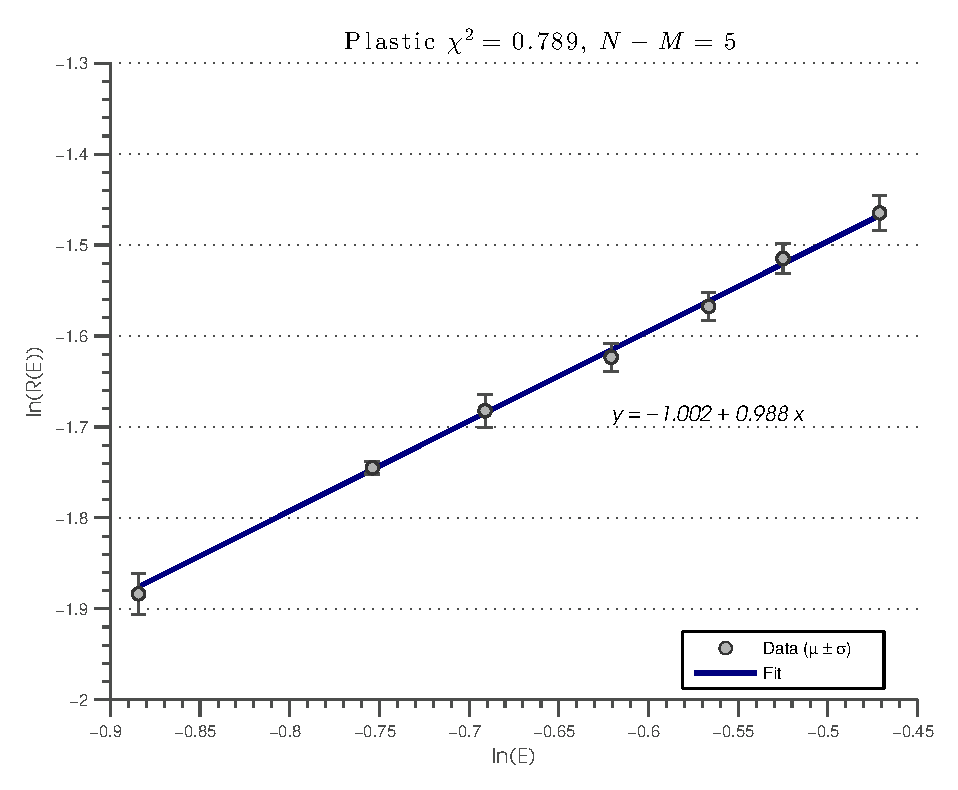
\includegraphics[width=\MyWidth]{Figures/linearPlasticGraph.eps}
  \caption{Graph of plastic data. $\ln(R(E))$ vs $\ln(E)$}
  \label{fig:Figures_linearPlasticGraph}
\end{figure}%(fig:Figures_linearPlasticGraph)


% section results (end)




\section{Discussion/Conclusion}

% (fold)
\label{sec:discussion_conclusion} The relative intensities between each plot of Figure~\ref{fig:Figures_aluminumShiftsPlot} do not give as much insight as those in Figure~\ref{fig:Figures_plasticShiftsPlot} because the counts collected were not declared beforehand. We realised the necessity of this criteria and set it for all the collected data with plastic. The data we collected agrees within our calculated error of uncertainty for higher energies, but for lower energies, our model gets progressively worse. 

We do expect to have a larger deviation at lower energies because we assumed a linear model to simplify calculations. It is also evident from both sources that the relationship isn't exactly linear, but roughly follows this semi-empirical equation from Katz and Penfold,\cite{RevModPhys.24.28} 
\begin{equation}
	R(E) = 0.412 E^{1.265 - 0.0954 \ln(E)} 
	\label{eq:acceptedEq} 
\end{equation} %(eq:acceptedEq)
Comparing this to our approximation, $R(E) = \kaluminum E^{\Baluminum}$ for aluminium and $\kplastic E^{\Bplastic}$ for plastic, we are satisfied with the results as they are good approximations.  It is good that the aluminum and plastic fitted equations agree with their NIST counterparts, even though the units for $R(E)$ is supposed to make it independent of the absorbing material. To calculate the errors, we used the equation,\cite{093570275X} $\delta R(E) = |k| \delta E$ and we know $\delta E$ from Table~\ref{tab:dataCollected}. Note that in this experiment, we assume that the uncertainty in the thickness of aluminium and plastic is negligible. 

In both Equation~\eqref{eq:acceptedEq} and our approximation, $R(E)$ is in units of $[\frac{\text{g}}{\text{cm}^2}]$ and E is in $[\text{MeV}]$. The uncertainty of our data is shown in Table~\ref{tab:uncertaintyConversion}. Berger states the uncertainty in measurements increases for lower energies, 
\begin{equation}
	\frac{\delta R(E)}{R(E)} = 
	\begin{cases}
		& 5 \text{~to~} 10~\% \text{ if } 10~\text{keV}<E<100~\text{keV} \\
		& 1 \text{~to~} 2~\% \text{ if } E>100~\text{keV} 
	\end{cases}
	\label{eq:bergerUncertainty}
\end{equation}
for the reason that at lower energies the electron energy is not large compared to the atomic electrons and therefore, the model, lacking any electron shell corrections, becomes less accurate. Berger also states that materials of low atomic number like air or plastic, will have a higher uncertainty $\sim 10\%$. In both of our models, we estimated about 1\% uncertainty, which likely means that we did not estimate our errors properly.
\begin{table}[h] 
   \begin{center} 
      \begin{tabular}{llll}\toprule 
\multicolumn{2}{c}{Aluminum} & \multicolumn{2}{c}{Plastic}\\ 
\cmidrule(r){1-2} 
\cmidrule(r){3-4} 
$\delta R(E)$ [$\frac{\text{mg}}{\text{cm}^2}$] & $\delta E$ [keV] & $\delta R(E)$ [$\frac{\text{mg}}{\text{cm}^2}$] & $\delta E$ [keV]\\ \midrule 
    2.32 &     5.50 &     2.04 &     4.00 \\ 
    2.23 &     5.50 &     1.94 &     4.00 \\ 
    2.13 &     5.50 &     0.76 &     1.50 \\ 
    2.40 &     6.50 &     3.26 &     7.50 \\ 
    3.25 &     9.00 &     0.59 &     1.50 \\ 
    1.52 &     4.50 &     3.60 &     8.50 \\ 
    4.48 &    13.00 &     4.32 &    10.50 \\ \bottomrule 
      \end{tabular} 
   \end{center}
\caption{The uncertainties in the range is calculated from our uncertainties in energy peaks using equation,\cite{093570275X} $\delta R(E) = |k| \delta E$. This equates to about 1 percent uncertainty.} 
\label{tab:uncertaintyConversion} 
\end{table} 

%(tab:uncertaintyConversion)

  
If we assume that our uncertainty in both E and R(E) also increase for lower energies, then our results almost agree within margins of error with the accepted model for all values of R(E) and E.  We believe that the fact that the equation for R(E) is independent of material shows us that our measurements for both materials were consistent with each other because they are within our estimated margins of error.  This lead us to believe that we would need a better approximation if we would want to improve our model to compare with other standards.  We also believe that our uncertainty was too low and it should on the same scale as other sources, 5\% to 10\%.

% The linear approximation was done because as more sheets of an absorber are added, the peaks become less distinguishable, meaning higher uncertainty in our measurements. 
% section discussion_conclusion (end)

\newpage
\bibliographystyle{IEEEtran}
\bibliography{Atomic_Nucleus}
%\noindent Updated \today.}
\end{document} 
